% Block Diagram for TTL IC Multiplexer 74HC153
% Author: Ramón Jaramillo.
\documentclass[tikz,border=10pt,12pt,x11names]{standalone}
%%%<
\usepackage{verbatim}
%%%>
\begin{comment}
:Title: Block Diagram for TTL IC Multiplexer 74HC153
:Tags: Circuits;Electrical engineering
:Author: Ramón Jaramillo
:Slug: multiplexer

This image was taken from a handbook about TTL Logic devices.
\end{comment}
\usepackage{tikz}
\usetikzlibrary{circuits.logic.US} % TiKZ Library for US Logic Circuits.
\begin{document}
	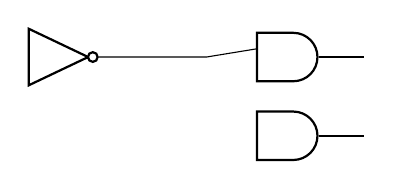
\begin{tikzpicture}[circuit logic US, every circuit symbol/.style={thick}]
	% Logic Gates
	\node[and gate,inputs={nn}, point right] (and1) at (2,-1)    {};
	\node[and gate,inputs={nn}, point right] (and2) at (2,-2)    {};
	\node[not gate, point right]               (not1) at (-1,-1) {};
	
	
	\draw (not1.output) -| (1,-1) -- (and1.input 1);
	
	%Outputs
	\draw (and1.output) [thick]-- (3,-1);
	\draw (and2.output) [thick]-- (3,-2);
	
	
	
	
	
	\end{tikzpicture}
\end{document}